\documentclass{standalone}
\usepackage{preset}
\begin{document}
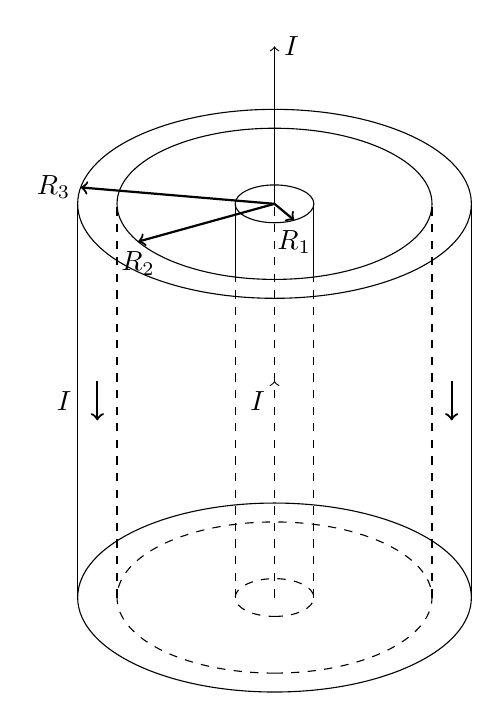
\begin{tikzpicture}[x={(-90:12mm)},y={(0:25mm)},z={(90:25mm)}]
	\draw[dashed](0,0,0)circle(.2);
	\draw[dashed](0,0,0)circle(.8);
	\draw(0,0,0)circle(1);
	\draw(0,0,2)circle(.2);
	\draw(0,0,2)circle(.8);
	\draw(0,0,2)circle(1);
	\draw[->,dashed](0,0,0)--node[left]{$I$}(0,0,2) (0,0,0)--(0,0,1.1);
	\draw[->](0,0,2)--++(0,0,.8)node[right]{$I$};
	\draw(0,.2,2)--+(0,0,-.38);
	\draw[dashed](0,.2,0)--+(0,0,2);
	\draw(0,-.2,2)--+(0,0,-.38);
	\draw[dashed](0,-.2,0)--+(0,0,2);
	\draw[dashed](0,.8,0)--+(0,0,2);
	\draw[dashed](0,-.8,0)--+(0,0,2);
	\draw(0,1,0)--+(0,0,2);
	\draw(0,-1,0)--+(0,0,2);
	\draw[thick,->](0,.9,1.1)--+(0,0,-.2);
	\draw[thick,->](0,-.9,1.1)--node[left=2mm]{$I$}+(0,0,-.2);
	\draw[thick,->](0,0,2)--+(30:.2)node[below]{$R_1$};
	\draw[thick,->](0,0,2)--+(-60:.8)node[below]{$R_2$};
	\draw[thick,->](0,0,2)--+(-100:1)node[left]{$R_3$};
\end{tikzpicture}
\end{document}
